% Drawing 154/05-1 -- folder 154, batch 05, archive page 82 (PDF page 83).
% Transcription: page de dessins en couleur, sans texte : quatre disques (bords vert clair), chacun traversé d'un arrangement de pseudo-droites tracées en brun, orange, gris et bleu, certaines en pointillé ; dans les deux disques du haut, des régions triangulaires près du bord et au centre sont coloriées en orange, et, dans celui de droite, des bandes sont hachurées en bleu ; dans les deux disques du bas, une bande en zigzag (gris foncé, hachurée) traverse l'arrangement de haut en bas, et deux points opposés du bord sont marqués. À gauche, un petit croquis d'un chemin en bleu et gris coupé de segments, et quelques traits de couleur (essais de feutres)
% Kind: four disks with coloured arrangements; zigzag bands; a small path sketch. Method 2 (schematic redraw from the facsimile). Status: partial.
% Notes: Page of drawings in colour, no text: four disks with light green rims, each crossed by an arrangement of pseudolines in brown, orange, grey and blue, some dotted; in the two upper disks triangular regions near the rim and at the centre are coloured orange (drawn as wedges at the rim) and in the right one bands are hatched in blue (left out); in the two lower disks a zigzag band (dark grey, hatched) crosses the arrangement from top to bottom, and two opposite points of the rim are marked. On the left a small sketch of a path in blue and grey cut by segments, and a few strokes of colour (pen trials). Disks, bands and marked points placed from the page view; the arrangements are schematic.
% Coordinates: 1 unit = 1 mm = 1/100 of the crop width (bbox in page fractions: [0.116, 0.082, 0.878, 0.502]).
% Redrawn by Claude (claude-opus-5-5), issue #73, 2026-11-07; not checked by a human; not compiled (no TeX in the session).
% Rights: reproduces part of the work -- behind RENDER_TRANSCRIPTS, never published by itself.
\documentclass[tikz,border=3pt]{standalone}
\usepackage{amsmath,amssymb}
\usetikzlibrary{patterns,arrows.meta}
\tikzset{Or/.style={orange!90!black}, Ye/.style={yellow!80!orange}, Lg/.style={green!60!black!70}, Dg/.style={green!45!black}, Br/.style={brown!80!black}, Rd/.style={red!85!black}, Bl/.style={blue!70!black}, Gy/.style={black!40}, pencil/.style={black!45}, struck/.style={black!35}, mark/.style={circle,draw,inner sep=1.3pt}, pt/.style={circle,fill,inner sep=0.9pt}, opt/.style={circle,draw,fill=white,inner sep=1.1pt}}
\begin{document}
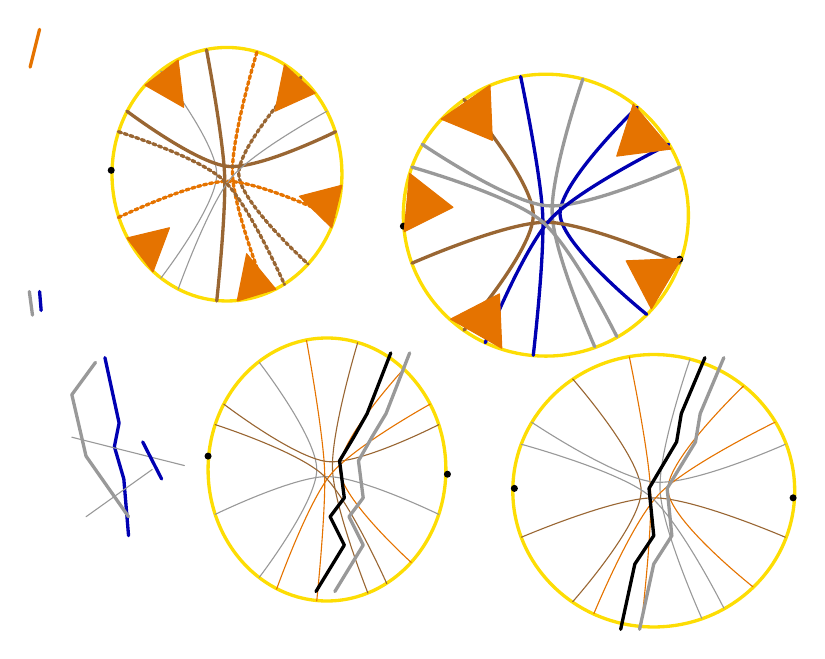
\begin{tikzpicture}[x=1mm,y=1mm,line cap=round,line join=round,font=\scriptsize]
\draw[Ye,very thick] (26.2,-19) ellipse[x radius=14.6, y radius=16.1];
\draw[Br,very thick] plot[smooth, tension=0.55] coordinates {(23.6,-3.2) (25.9,-19.1) (24.9,-35.1)};
\draw[Or,densely dotted,very thick] plot[smooth, tension=0.55] coordinates {(30,-3.5) (26.9,-19) (31.2,-34.1)};
\draw[Gy] plot[smooth, tension=0.55] coordinates {(17.8,-5.9) (24.9,-19) (17.8,-32.2)};
\draw[Br,densely dotted,very thick] plot[smooth, tension=0.55] coordinates {(35.6,-6.7) (27.7,-19) (36.5,-30.4)};
\draw[Br,very thick] plot[smooth, tension=0.55] coordinates {(13.5,-11) (26.3,-18) (40,-13.6)};
\draw[Or,densely dotted,very thick] plot[smooth, tension=0.55] coordinates {(12.4,-24.5) (26.2,-19.9) (40,-24.5)};
\draw[Gy] plot[smooth, tension=0.55] coordinates {(38.9,-11) (26.7,-19.5) (20,-33.6)};
\draw[Br,densely dotted,very thick] plot[smooth, tension=0.55] coordinates {(12.4,-13.6) (25.7,-19.7) (33.5,-33)};
\node[pt] at (11.5,-18.5) {};
\draw[Or] (20,-4.5) -- (15.8,-7.7) -- (20.7,-10.5) -- cycle;
\fill[pattern=north east lines,Or] (20,-4.5) -- (15.8,-7.7) -- (20.7,-10.5) -- cycle;
\draw[Or] (37.4,-8.7) -- (33.5,-5.1) -- (32.3,-11) -- cycle;
\fill[pattern=north east lines,Or] (37.4,-8.7) -- (33.5,-5.1) -- (32.3,-11) -- cycle;
\draw[Or] (39.5,-25.8) -- (40.8,-20.4) -- (35.4,-21.8) -- cycle;
\fill[pattern=north east lines,Or] (39.5,-25.8) -- (40.8,-20.4) -- (35.4,-21.8) -- cycle;
\draw[Or] (27.5,-35.1) -- (32.4,-33.6) -- (28.7,-29.1) -- cycle;
\fill[pattern=north east lines,Or] (27.5,-35.1) -- (32.4,-33.6) -- (28.7,-29.1) -- cycle;
\draw[Or] (13.5,-27.1) -- (16.8,-31.4) -- (18.9,-25.8) -- cycle;
\fill[pattern=north east lines,Or] (13.5,-27.1) -- (16.8,-31.4) -- (18.9,-25.8) -- cycle;
\draw[Ye,very thick] (66.7,-24.2) ellipse[x radius=18.1, y radius=17.9];
\draw[Bl,very thick] plot[smooth, tension=0.55] coordinates {(63.5,-6.6) (66.3,-24.2) (65.1,-42)};
\draw[Gy,very thick] plot[smooth, tension=0.55] coordinates {(71.4,-6.9) (67.5,-24.1) (72.9,-40.9)};
\draw[Br,very thick] plot[smooth, tension=0.55] coordinates {(56.3,-9.5) (65.1,-24.2) (56.3,-38.8)};
\draw[Bl,very thick] plot[smooth, tension=0.55] coordinates {(78.3,-10.5) (68.5,-24.1) (79.5,-36.8)};
\draw[Gy,very thick] plot[smooth, tension=0.55] coordinates {(51,-15.2) (66.8,-23) (83.7,-18.1)};
\draw[Br,very thick] plot[smooth, tension=0.55] coordinates {(49.7,-30.3) (66.7,-25.1) (83.7,-30.3)};
\draw[Bl,very thick] plot[smooth, tension=0.55] coordinates {(82.3,-15.2) (67.3,-24.7) (59,-40.4)};
\draw[Gy,very thick] plot[smooth, tension=0.55] coordinates {(49.7,-18.1) (66.1,-24.9) (75.7,-39.6)};
\node[pt] at (48.6,-25.6) {};
\node[pt] at (83.7,-29.8) {};
\draw[Or] (59.6,-7.7) -- (53.4,-12) -- (59.9,-14.7) -- cycle;
\fill[pattern=north east lines,Or] (59.6,-7.7) -- (53.4,-12) -- (59.9,-14.7) -- cycle;
\draw[Or] (82.6,-15.8) -- (77.8,-10.1) -- (75.7,-16.7) -- cycle;
\fill[pattern=north east lines,Or] (82.6,-15.8) -- (77.8,-10.1) -- (75.7,-16.7) -- cycle;
\draw[Or] (49.4,-18.9) -- (48.7,-26.3) -- (54.9,-23.2) -- cycle;
\fill[pattern=north east lines,Or] (49.4,-18.9) -- (48.7,-26.3) -- (54.9,-23.2) -- cycle;
\draw[Or] (80.1,-36.1) -- (83.9,-29.7) -- (76.9,-30) -- cycle;
\fill[pattern=north east lines,Or] (80.1,-36.1) -- (83.9,-29.7) -- (76.9,-30) -- cycle;
\draw[Or] (54.6,-37.4) -- (61.1,-41.1) -- (60.8,-34.2) -- cycle;
\fill[pattern=north east lines,Or] (54.6,-37.4) -- (61.1,-41.1) -- (60.8,-34.2) -- cycle;
\draw[Ye,very thick] (38.9,-56.5) ellipse[x radius=15.1, y radius=16.7];
\draw[Or] plot[smooth, tension=0.55] coordinates {(36.3,-40.1) (38.6,-56.6) (37.6,-73.2)};
\draw[Br] plot[smooth, tension=0.55] coordinates {(42.8,-40.4) (39.6,-56.5) (44.1,-72.2)};
\draw[Gy] plot[smooth, tension=0.55] coordinates {(30.3,-42.9) (37.6,-56.5) (30.3,-70.2)};
\draw[Or] plot[smooth, tension=0.55] coordinates {(48.6,-43.8) (40.5,-56.5) (49.6,-68.3)};
\draw[Br] plot[smooth, tension=0.55] coordinates {(25.8,-48.2) (39,-55.5) (53.1,-50.8)};
\draw[Gy] plot[smooth, tension=0.55] coordinates {(24.7,-62.2) (38.9,-57.4) (53.1,-62.2)};
\draw[Or] plot[smooth, tension=0.55] coordinates {(52,-48.2) (39.4,-57.1) (32.5,-71.7)};
\draw[Br] plot[smooth, tension=0.55] coordinates {(24.7,-50.8) (38.4,-57.2) (46.5,-71)};
\draw[very thick] (47,-41.7) -- (44,-49.4) -- (42.3,-52.4) -- (40.5,-55.4) -- (41.1,-60.1) -- (39.3,-62.5) -- (41.1,-66.1) -- (37.5,-72);
\draw[Gy,very thick] (49.4,-41.7) -- (46.4,-49.4) -- (44.6,-52.4) -- (42.9,-55.4) -- (43.5,-60.1) -- (41.7,-62.5) -- (43.5,-66.1) -- (39.9,-72);
\node[pt] at (23.8,-54.8) {};
\node[pt] at (54.2,-57.1) {};
\draw[Ye,very thick] (80.4,-59.2) ellipse[x radius=17.9, y radius=17.3];
\draw[Or] plot[smooth, tension=0.55] coordinates {(77.3,-42.2) (80,-59.2) (78.8,-76.4)};
\draw[Gy] plot[smooth, tension=0.55] coordinates {(85,-42.5) (81.2,-59.1) (86.5,-75.4)};
\draw[Br] plot[smooth, tension=0.55] coordinates {(70.1,-45) (78.8,-59.2) (70.1,-73.3)};
\draw[Or] plot[smooth, tension=0.55] coordinates {(91.8,-45.9) (82.2,-59.1) (93,-71.4)};
\draw[Gy] plot[smooth, tension=0.55] coordinates {(64.9,-50.5) (80.5,-58.1) (97.1,-53.3)};
\draw[Br] plot[smooth, tension=0.55] coordinates {(63.6,-65.1) (80.4,-60.1) (97.1,-65.1)};
\draw[Or] plot[smooth, tension=0.55] coordinates {(95.8,-50.5) (81,-59.7) (72.8,-74.8)};
\draw[Gy] plot[smooth, tension=0.55] coordinates {(63.6,-53.3) (79.8,-59.8) (89.3,-74.1)};
\draw[very thick] (86.9,-42.3) -- (83.9,-49.4) -- (83.3,-53) -- (79.8,-58.9) -- (80.4,-64.9) -- (78,-68.5) -- (76.2,-76.8);
\draw[Gy,very thick] (89.3,-42.3) -- (86.3,-49.4) -- (85.7,-53) -- (82.1,-58.9) -- (82.7,-64.9) -- (80.4,-68.5) -- (78.6,-76.8);
\node[pt] at (62.7,-58.9) {};
\node[pt] at (98.1,-60.1) {};
\draw[Bl,very thick] (10.7,-42.3) -- (12.5,-50.6) -- (11.9,-53.6) -- (13.1,-57.7) -- (13.7,-64.9);
\draw[Gy,very thick] (9.5,-42.9) -- (6.5,-47) -- (8.3,-54.8) -- (13.7,-62.5);
\draw[Gy] (6.5,-52.4) -- (20.8,-56);
\draw[Gy] (8.3,-62.5) -- (16.7,-56.5);
\draw[Bl,very thick] (15.5,-53) -- (17.9,-57.7);
\draw[Or,very thick] (1.2,-5.4) -- (2.4,-0.6);
\draw[Gy,very thick] (1.1,-33.9) -- (1.5,-36.9);
\draw[Bl,very thick] (2.4,-33.9) -- (2.6,-36.3);
\end{tikzpicture}
\end{document}
